\chapter{Image manipulation}
\vspace{-10mm}

Dicom-Presenter is an application for viewing image data. Entire image manipulation was solved with use of OpenGL library in early version of Dicom-Presenter. OpenGL was used for image storing, for changing image properties and for drawing images on screen. Unfortunately, OpenGL brought complications to application compatibility with various hardware. Therefore, author of this work decided to remove OpenGL from application and replace all classes using OpenGL with their non-OpenGL equivalents. 

Before rewriting all image processing classes without OpenGL it was a need to study how to complete all image processing tasks without OpenGL. Moreover, OpenGL uses GPU to perform it's tasks so it was a need to calculate the loss of performance when OpenGL will be removed. 

\section{Image storing}
As a part of rendering engine reimplementation it was mandatory to understand how are image data stored in computer memory. A color image consisting of $m \cdot n$ points (pixels) can be described by $m \cdot n$ number triads. The triads would be coordinates in RGB or HSV color space \footnote{All visible colors can be decomposed into three independent components due to the fact that human eye contains three different color receptors. }. Data in a computer are stored in elementary units - bytes, which can hold 256 different values. Each byte consists of eight unitary units - bits ($2^8 = 256 $). If considered that one byte can include color information of only one pixel, then only eight-bit multiples can be used for a pixel color storage: 8 bits, 16 bits, 24 bits, etc. In case of 24 bit color depth, three bytes are used for a pixel color storage - each byte for each color. If 8 bits depth or 16 bits depth is used, in both cases the bit numbers are not divisible by three, so there are several ways of how to distribute bits among colors.
 
Qt library uses three diferent formats of 16 bit color information storage. The formats differ by number of bits distributed to each color and are described by triads of numbers: 5-6-5, 5-5-5, 4-4-4. The first format uses 5 bits for red color, 6 bits for green color and 5 bits for blue color. The numbers of bits for each color are uneven but no redundant bits are present. Both 5-5-5 and 4-4-4 formats include redundant bits for each image pixel.

Qt library allows displaying images which are actually saved in computer memory as an array of bytes in some of supported formats (such as described above). Besides color depth formats, image storage can differ by number of bytes used for storing each image line. If an image has $m \cdot n$ pixels and two bytes are used per pixel (f.e. 16 bit 5-5-5), there is no rule that $m \cdot n \cdot 2$ bytes will be used. A computer memory in x86 architecture reads its data in elements called words usually consisting of 4 bytes for x86 architecture and 8 bytes for 64-bit architecture. Therefore, image data are in computer memory often aligned that each image line starts at a beginning of some 4-byte or 8-byte word. For instance, if we consider an image of $100 \cdot 100$ pixels saved with 8 bit pixel depth on 64-bit architecture, each line consisting of $100$ pixels would be saved on $128$ or bytes.

In conclusion, if a picture is reconstructed from uncompressed raw data saved in computer memory, essential indications are which color storage format is used for each pixel and which bit align is used for each pixel-line. Those two information are enough for correct image reconstruction.

\subsection{Image construction from raw data in Qt library}



\begin{figure}
	\begin{center}
	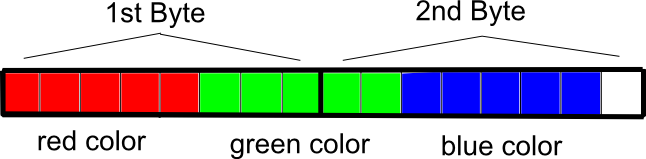
\includegraphics[width=130mm]{Text/IMG/ImageStoring_16bit.png}
	\end{center}
	\caption{A distribution of 16 bits of 2 bytes among three colors of a pixel.}
	\label{screenshot}
\end{figure}

\section{Image enhancement operations}

One of important tasks to reimplement in Dicom-Presenter was an ability to adjust image brightness and contrast. Images which will be opened in Dicom-Presenter can be captured on various MRI units with various imaging properties. The ability to increase image brightness and contrast is mandatory to ensure sufficient display quality. Too dark or too gray images need to be brightened or need to increase contrast to ensure better observation of physiological findings. A brightness and contrast change is among DICOM users called ``windowing''.

For further needs of this text let's define brightness and contrast. 

A grayscale image can be considered as a matrix of numbers: 

\[
 Im_{res_{x},res_{y}} =
 \begin{pmatrix}
  Im(1,1) & Im(1,2) & \cdots & Im(1,res_{x}) \\
  Im(2,1) & Im(2,2) & \cdots & Im(2,res_{x}) \\
  \vdots  & \vdots  & \ddots & \vdots  \\
  Im(res_{y},1) & Im(res_{y},2) & \cdots & Im(res_{y},res_{x})
 \end{pmatrix}
\]

where $ res_{x} $, $res_{y}$ are dimensions of the image. $Im(x,y)$ is a lightness of a pixel.

Brightness then can be defined as:
\[
  Brightness(Im) = \frac{1}{res_{x}  \cdot res_{y}}\sum_{\substack{0 \leq x \leq res_{x} \\ 0 \leq y \leq res_{y}}} Im(x,y)
\]

Contrast is understood as overall difference in luminosity between bright and dark pixels. There are more possible definitions of contrast. One possible definition is:

\[
Contrast(Im) = \sqrt{\frac{1}{res_{x} \cdot res_{y}}\sum_{\substack{ 0 \leq x \leq res_{x} \\ 0 \leq y \leq res_{y} }}(Im_{x,y}-Brightness(Im))^2}
\]

An argument for using these two definitions for brightness and contrast is that they are analogies for mean value and variance of set of values.

If there is a need of increasing or decreasing image brightness in computer applications simply a constant id added to all image points:

\begin{equation}
\label{brightness}
  Im(x,y) \longmapsto Im(x,y) + c_{brightness} 
\end{equation}

Image contrast is usually adjusted by a linear transformation applied to all image points:

\begin{equation}
\label{contrast}
  Im(x,y) \longmapsto   (Im(x,y) - 0.5) \cdot c_{contrast} + 0.5
\end{equation}

A disadvantage of both ways is that some image information is lost. Let's consider an image described by a matrix with elements of integers in range from zero to 255. Let the brightness of the picture increased according to formula \eqref{brightness} with a positive constant $ c_{brightness} $. Then all the points brighter than $ 255 - c_{brightness} $ on original image will have luminosity of 255 regardless their original luminosity. Similarly if contrast would be increased according to formula \eqref{contrast} with a constant $ c_{contrast} $ then all points brighter than $ \frac{1}{2} \cdot 255 \cdot (\frac{1}{c_{contrast}}+1) $ will have the same color (maximum white). As well all pixels darker than $ \frac{1}{2} \cdot 255 \cdot (1 - \frac{1}{c_{contrast}}) $ will have the same color (maximum black).

\clist{krivka na nelinearni kontrast z vyzkumaku}

\subsection{Pixel manipulations in Qt}



\section{Image rendering}


\red{
Renderovani snimku na ruzna mista na obrazovce pomoci Qt.\\
Ukazat bezpecny zpusob pomoci Qt.\\
Ukazat nebezpecny zpusob pomoci primych zasahu do pameti.\\
Zduvodnit proc se radeji priklonime k prehlednemu a bezpecnemu zpusobu pomoci Qt.\\
Zpisob primeho zapisu do pameti at dela jiny student - je to prace na cca pul roku, ale pujde krasne navazat na moji verzi DP.\\
}

\section{OpenGL and Qt performance}

\red{
Ukazat mereni performance a ukazat vzorecek na odhad rychlosti vykreslovani.\\
}